
\documentclass{article}

\usepackage{graphicx}
\usepackage{apacite}
\usepackage{natbib}
\usepackage[linktocpage]{hyperref}
\usepackage[fleqn]{amsmath}
\usepackage{mathtools}
\usepackage{amsthm}
\usepackage{amssymb}
\usepackage{verbatim}
\usepackage{lineno}

\allowdisplaybreaks
\linenumbers

\DeclarePairedDelimiterX{\inp}[2]{\langle}{\rangle}{#1, #2}

\theoremstyle{lemma}
\newtheorem{lemma}{Lemma}

\begin{document}

\title{Comments on \emph{Section 6.1.3 Supercritical Andronov-Hopf} of
\citet{izhikevich07}}
\author{Joaqu\'{i}n Rapela\thanks{rapela@ucsd.edu}}
\maketitle

\tableofcontents

\section{Introduction}

The book \citet{izhikevich07} is excellent. 
However, when I reached \emph{Section 6.1.3 Supercritical Andronov-Hopf} I did
not feel comfortable with the presentation of a few formulas without derivation or explanation of where these formulas came from or what do they meant.
Specifically, I could not understand the rationale for the change of variables
in Equation~6.5, where the formula for parameter $a$ in Equation~6.7 came
from or what did it mean, how to derive the topological normal form in
Equations~6.8 and 6.9, and how to compute parameter $d$ in Equation~6.9.

Here I sketch the derivation of the topological normal form in Equations~6.8
and 6.9 and that of the formulas to calculate parameters $a$ and $d$ in
these equations.  In deriving the topological normal in Equations~6.8 and
6.9, I found that these equations do not represent a true topological normal
form of a system undergoing an Andronov-Hopf bifurcation, but only an
\emph{approximation} of a true topological normal form.  The formula for
parameter $a$ is given, without proof in Equation~6.7. On page 172 the
author refers the reader to Exercise 6.17 to obtain the values of parameters
$a$ and $d$ for an example $I_{N_{a,p}}+I_K$ model. However, this exercise
gives neither the formula nor the value of parameter $d$.  Furthermore,
applying the formulas we derive below for parameters $a$ and $d$ to the
example $I_{N_{a,p}}+I_K$ model on page 172 reveals a typo; the values of
parameters $a$ and $d$ are interchanged in the penultimate paragraph on page 172,
in the subsequent formula of the topological normal form of the
$I_{N_{a,p}}+I_K$ model, and the center and right panels of Figure 6.12 were
computed with interchanged parameters.

Section~\ref{sec:sketchDerivation6_8and6_9} provides a sketch of the
derivation of the \emph{approximate} topological normal form in Equations~6.8 
and 6.9.
% Section~\ref{sec:rationaleChangeOfVariablesIn6_5} provides a rationale for
% choosing the change of variables given in Equation~6.5 demonstrates why this change of variables leads to the
% system of differential equations in Equation~6.6,
% and derives the formulas for the function $f(x,y)$ and $g(x,y)$ appearing in
% Equation~6.6.
Section~\ref{sec:sketchDerivationFormulaParametersAandD} sketches the
derivation of the formulas of parameters $a$ and $d$ of the topological normal
form for a system undergoing an Andronov-Hopf bifurcation.  
%
Section~\ref{sec:derivationFormulas_fg} derives the formulas for $f(x,y)$ and
$g(x,y)$ in Equation~6.6.
%
Section~\ref{sec:adExampleP172} calculates the values of parameters $a$ and
$d$ for the example on page 172.
%
Finally, Section~\ref{sec:evidenceForTypoPage172} presents evidence for the
typo in the example on page 172.

\section{Sketch of the derivation of the \emph{approximate} topological normal
form in Equations~6.8 and 6.9 of
\citet{izhikevich07}}
\label{sec:sketchDerivation6_8and6_9}

Consider a planar system 

\begin{align}
 \mathbf{\dot{x}}=f(\mathbf{x},\alpha),\; \mathbf{x}\in \mathbb{R}^2,\; \alpha\in \mathbb{R}
 \label{eq:systemUndergoingAHBifurcation}
\end{align}

\noindent with a smooth function $f$, and an equilibrium at $\mathbf{x}=0$ for
parameter $\alpha=0$. This system undergoes and Andronov-Hopf
bifurcation iff its eigenvalues are $\lambda_{1,2}=\pm jw_0, w_0>0$. From
Section 3.5 Generic Hopf Bifurcation of \citet{kuznetsov04} a planar system
undergoing an Andronov-Hopf bifurcation can be
rewritten as

\begin{align}
 \mathbf{\dot{x}}=A(\alpha)\mathbf{x}+F(\mathbf{x},\alpha)
 \label{eq:k311}
\end{align}

\noindent where $F$ is a smooth vector function whose components $F_{1,2}$
have Taylor expansions in $\mathbf{x}$ starting with at least quadratic terms
$F=\mathcal{O}(||\mathbf{x}||^2)$. Then, by Lemma 3.3 in~\citet{kuznetsov04},
the system in Equation~\ref{eq:k311} can be rewritten for sufficiently small
$|\alpha|$ a single complex equation

\begin{align}
 \dot{z}=\lambda(\alpha)z+g(z,\bar{z},\alpha),
 \label{eq:k312}
\end{align}

\noindent where $g=\mathcal{O}(|z|^2)$ is a smooth function of
$(z,\bar{z},\alpha)$. Now from Lemma 3.6 (Poincar\'{e} normal form for the
Hopf bifurcation) in \citet{kuznetsov04} Equation~\ref{eq:k312} can be
transformed, by an invertible parameter-dependent change of complex
coordinate, for sufficiently small $|\alpha|$, into

\begin{align}
 \dot{w}=\lambda(\alpha)w+c_1(\alpha)w^2w+\mathcal{O}(|w|^4).
 \label{eq:k316}
\end{align}

Denoting $\lambda(\alpha)=c(\alpha)+jw(\alpha)$ and
$c_1(\alpha)=a(\alpha)+jd(\alpha)$, by Problem 6.4 in \citet{izhikevich07},
the complex-valued Equation~\ref{eq:k316} can be written in polar coordinates
as

\begin{equation}
 \begin{aligned}
  \dot{r}&=c(\alpha)r+a(\alpha)r^3,\\
  \dot{\varphi}&=w(\alpha)+d(\alpha)r^2
 \end{aligned}
 \label{eq:trueNormalForm}
\end{equation}

The system in Equation~\ref{eq:trueNormalForm} is a true topological normal
form of the sytem in Equation~\ref{eq:systemUndergoingAHBifurcation}
undergoing an Andronov-Hopf bifurcation, because the former system can be
obtained from the latter system by a change of variables that is an
homeomorphism. However, the topological normal form in Equations~6.8 and
6.9 of \citet{izhikevich07} is an approximation of the true toplogical
normal form using $a(0)$ and $d(0)$ instead of $a(\alpha)$ and $d(\alpha)$ in
Equation~\ref{eq:trueNormalForm}.

To obtain exact values of $a$ and $d$ independent of any parameter, one could
use a topological normal form as in Equation~\ref{eq:k316} but with a
coefficient of the cubic term independent of any parameter (e.g.,
$c_1(\alpha)=c_1$ in Equation~\ref{eq:k316}). This new topological normal form
is given in Lemma~3.7 of \citet{kuznetsov04}. In this lemma \citet{kuznetsov04}
attains a topological normal form where the coefficient of the cubic term is
$\textrm{sign}(l_1(\beta))$. Because $l_1(\beta)$ is a continuous function of
$\beta$, with $l_1(0)\neq 0$, for small values of $\beta$ the $\textrm{sign}$
of $l_1(\beta)$ is constant (i.e., $\textrm{sign}(l_1(\beta))=s$).  Therefore,
by replacing $\textrm{sign}(l_1(\beta))$ with $s$ in the previous topological
normal form, for small values of $\beta$, Kuznetsov attains a new topological
normal form with the coefficient of the cubic term independent of any
parameter.

\section{Sketch of derivation of formulas for parameters $a$ and $d$ in
Equations~6.8 and 6.9 of \citet{izhikevich07}}
\label{sec:sketchDerivationFormulaParametersAandD}

As shown by the end of Section~\ref{sec:sketchDerivation6_8and6_9} parameters
$a$ and $d$ in Equations~6.8 and 6.9 of \citet{izhikevich07} are
$a=Re\{c_1(0)\}$ and $d=Im\{c_1(0)\}$, with $c_1(0)$ given in
Equation~\ref{eq:k316}. To calculate $c_1(0)$ we first apply the change
of variables in Equation~6.5 of \citet{izhikevich07} to convert the system
undergoing an Andronov-Hopf bifurcation in Equation~6.4 of
\citet{izhikevich07}, with parameter $b=0$, into the form in Equation~6.6 of
\citet{izhikevich07}. Then we solve Problem~(3.16) in \citet{kuznetsov04} to
obtain $c_1(0)$ from the system in Equation~6.6 of \citet{izhikevich07}.

Section~\ref{sec:rationaleEqs6_5And6_6} provides the rationale for
Equations~6.5 and 6.6 of \citet{izhikevich07}.
Section~\ref{sec:solutionProblem3.16InKuznetsov04} sketches the solution of
Problem 3.16 in \citet{kuznetsov04}.

\subsection{Rationale for Equations~6.5 and 6.6 in
\citet{izhikevich07}}
\label{sec:rationaleEqs6_5And6_6}

The rationale for the change of variables in Equation~6.5 of
\citet{izhikevich07} is given in Lemma 3.3 of \citet{kuznetsov04}. This lemma
proves that a system of differential equations

\begin{align}
\mathbf{\dot{x}}=A(\alpha)\mathbf{x}+F(\mathbf{x},\alpha)\nonumber
\end{align}

\noindent where $F:\mathbb{R}^2\times\mathbb{R}\rightarrow\mathbb{R}^2$ is a
smooth vector function whose components have Taylor expansions in $\mathbf{x}$
starting with at least quadratic terms, can be written as a single
differential equation on a complex variable $z$:

\begin{align}
\dot{z}=\lambda(\alpha)z+g(z,\bar{z},\alpha)
\label{eq:zDotKusnetzov}:
\end{align}

\noindent with $\lambda(\alpha)$ being the eigenvalue of $A(\alpha)$
corresponding to eigenvector $\mathbf{q}(\alpha)$ (i.e.,
$A(\alpha)\mathbf{q}(\alpha)=\lambda(\alpha)\mathbf{q}(\alpha)$) and $z$ being
the coordinate associated with $\mathbf{q}(\alpha)$ in the expansion of
$\mathbf{x}$ in the base $\{\mathbf{q}(\alpha),\mathbf{\bar{q}}(\alpha)\}$,

\begin{align}
\mathbf{x}=z\mathbf{q}(\alpha)+\bar{z}\mathbf{\bar{q}}(\alpha),
\label{eq:xExpandedOnz}
\end{align}

\noindent and 

\begin{align}
g(z,\bar{z},\alpha)=\inp{\mathbf{p}(\alpha)}{F(z\mathbf{q}(\alpha)+\bar{z}\mathbf{\bar{q}}(\alpha),\alpha)}\label{eq:gAtz}
\end{align}

\noindent with $\{\mathbf{p}(\alpha),\mathbf{\bar{p}}(\alpha)\}$ a base of
eigenvectors of $A(\alpha)^T$ biorthogonal with the base
$\{\mathbf{q}(\alpha),\mathbf{\bar{q}}(\alpha)\}$ of $A(\alpha)$.
The Taylor series expansion of the right-hand-side of the differential
equations in Equation~6.4 of \citet{izhikevich07}, for $b=0$
can be written as:

\begin{align}
\left[\begin{array}{c}
        \dot{v}\\
        \dot{u}
       \end{array}\right] = A(0) \left[\begin{array}{c}
                                         v\\
                                         u
                                        \end{array}\right] +
                            \left[\begin{array}{c}
                                    \tilde{F}(v, u, 0)\\
                                    \tilde{G}(v, u, 0)
                                   \end{array}\right]
\label{eq:6.4rewritten}
\end{align}

\noindent with $A(0)$ being the jacobian matrix of the right hand side of the
differential equations in Equation~6.4 of \citet{izhikevich07}

\begin{align}
A(0)=\left[\begin{array}{cc}
                F_u & F_v\\
                G_u & G_v
           \end{array}\right]
\label{eq:jacobian}
\end{align}

\noindent where $F_u,F_v,G_u,G_v$ are partial derivatives evaluated at
$(u,v,b)=(0,0,0)$. Equation~\ref{eq:6.4rewritten} holds because it is assummed
that $(v,u)=(0,0)$ is an equilibrium for $b=0$ of the system of differential
equations in Equation~6.4 of \citet{izhikevich07}, then
$F(0,0,0)=G(0,0,0)=0$, and the Taylor series expansion of the right-hand-side
of Equation~6.4 in \citet{izhikevich07} has no constant term.

Now, because it is assummed that the system in Equation~6.4 in
\citet{izhikevich07} undergoes an Andronov-Hopf bifurcation at the equlibrium
$(v,u)=(0,0)$, by the non-hyperbolicity condition of the Andronov-Hopf
bifurcation, the eigenvalues of $A(0)$
in Equation~\ref{eq:6.4rewritten} are $\pm jw$. Then by
Equation~\ref{eq:zDotKusnetzov}:

\begin{align}
    \dot{z}=jwz+g(z,\bar{z},0)
    \label{eq:zDot}
\end{align}

\noindent with 
$z$ being
the coordinate associated with $\mathbf{q}(0)$ in the expansion of
$[v,u]^T$ in the base $\{\mathbf{q}(0),\mathbf{\bar{q}}(0)\}$.
That is, from Equation~\ref{eq:xExpandedOnz},

\begin{align}
\left[\begin{array}{c}
        v\\
        u
       \end{array}\right]=z\mathbf{q}(0)+\bar{z}\mathbf{\bar{q}}(0)
\label{eq:vuExpandedOnz}
\end{align}

Separating the real and imaginary parts of z in Equation~\ref{eq:zDot} we
obtain:

\begin{align}
    Re\{\dot{z}\}&=-wIm\{z\}+Re\{g(z,\bar{z},0)\}\nonumber\\
    Im\{\dot{z}\}&=wRe\{z\}+Im\{g(z,\bar{z},0)\}\nonumber
\end{align}

\noindent and calling 

\begin{align}
x&=Re\{z\},\label{eq:x}\\
y&=Im\{z\},\label{eq:y}\\
f(x,y)&=Re\{g(z,\bar{z},0)\},\label{eq:f}\\
g(x,y)&=Im\{g(z,\bar{z},0)\}\label{eq:g},
\end{align}

\noindent we obtain

\begin{align}
    \dot{x}&=-wy+f(x,y)\nonumber\\
    \dot{y}&=wx+g(x,y\nonumber)
\end{align}

\noindent as in Equation~6.6 in \citet{izhikevich07}.

To express $x$ and $y$ as a function of $v$ and $u$, as in Equation~6.5 of
\citet{izhikevich07}, from Equations~\ref{eq:x} and~\ref{eq:y}, we want to
express $z$ as a function of $v$ and $u$. One can build the
biorthogonal base $\{\mathbf{p}(0),\mathbf{\bar{p}}(0)\}$ corresponding to the
base of eigenvectors of $A(0)$,
$\{\mathbf{q}(0),\mathbf{\bar{q}}(0)\}$ and, from
Equation~\ref{eq:vuExpandedOnz}, compute $z$ as

\begin{align}
z=\inp{\mathbf{p}(0)}{\left[\begin{array}{c}
                             v\\
                             u
                            \end{array}\right]}
\label{eq:z}
\end{align}

Because $\mathbf{\bar{q}}(0)$ is the
eigenvector of $A(0)$ (Equation~\ref{eq:jacobian}) with eigenvalue $-jw$, we have

\begin{align}
\left[\begin{array}{cc}
       F_v+jw&F_u\\
       G_v&G_u+jw
      \end{array}\right]
\left[\begin{array}{c}
       \bar{q}_1(0)\\
       \bar{q}_2(0)
      \end{array}\right]=0\nonumber
\end{align}

\noindent Then 

\begin{align}
(F_v+jw)\bar{q}_1(0)+F_u\bar{q}_2(0)=0
\label{eq:orthogonality}
\end{align}

\noindent Due to the
biorthogonality of the bases $\{\mathbf{p}(0),\mathbf{\bar{p}}(0)\}$ and
$\{\mathbf{q}(0),\mathbf{\bar{q}}(0)\}$ we have
$\inp{\mathbf{p}(0)}{\mathbf{\bar{q}}(0)}=0$. Thus, from
Equation~\ref{eq:orthogonality}, we obtain

\begin{align}
    \mathbf{p}(0)=k\left[\begin{array}{c}
                          F_v-jw\\
                          F_u
                         \end{array}\right]\label{eq:p}
\end{align}

\noindent where $k$ is a complex constant. Now, from Equations~\ref{eq:z}
and~\ref{eq:p}

\begin{align}
z=&\inp{\mathbf{p}(0)}{\left[\begin{array}{c}
                              v\\
                              u
                             \end{array}\right]}\nonumber\\
=&\bar{k}v(F_v+jw)+\bar{k}uF_u\nonumber\\
=&\bar{k}(uF_u+vF_v)+j\bar{k}wv\label{eq:zAsFvu}
\end{align}

By using $k=j/w$ in Equation~\ref{eq:zAsFvu} we obtain $z=v-j(uF_u+vF_v)/w$.
Then $x=Re\{z\}=v$, and $y=Im\{z\}=-(uF_u+vF_v)/w=-(uF_u+xF_v)/w$, or $v=x$
and $F_uu=-F_vx-wy$ as in Equation~5.5 of
\citet{izhikevich07}.

\subsection{Solution to Problem~3.16 in \citet{kuznetsov04}}
\label{sec:solutionProblem3.16InKuznetsov04}

Given a system as that in Equation~6.6 of \citet{izhikevich07}, Problem~3.16 in \citet{kuznetsov04}
asks to compute $c_1(0)$. The solution is $c_1(0)=a(0)+jd(0)=a+jd$ with

\begin{align}
a=&\frac{1}{16}((f_{xxx}+g_{xxy}+f_{xyy}+g_{yyy})+\nonumber\\
&\qquad\frac{1}{w}(g_{yy}f_{yy}-g_{xx}f_{xx}+f_{xy}(f_{xx}+f_{yy})-g_{xy}(g_{xx}+g_{yy}))),\label{eq:a}\\
d=&\frac{1}{16}((g_{xxx}+g_{xyy}-f_{xxy}-f_{yyy})+\nonumber\\
&\qquad\frac{1}{3w}((f_{xy}g_{xx}+g_{xy}f_{yy})-2(g_{yy}^2+f_{xx}^2)-2(f_{xy}^2+g_{xy}^2)-\nonumber\\
&\qquad\qquad5(g_{xx}^2+f_{yy}^2)+5(f_{xy}g_{yy}+g_{xy}f_{xx})-\nonumber\\
&\qquad\qquad5(g_{xx}g_{yy}+f_{xx}f_{yy})))\label{eq:d}.
\end{align}

To derive this solution, we first rewrite
Equation~6.6 of \citet{izhikevich07} in matrix form as

\begin{align}
\left[\begin{array}{c}
        \dot{x}\\
        \dot{y}
       \end{array}\right]&= A(0)\left[\begin{array}{c}
                                      x\\
                                      y
                                     \end{array}\right]+
                           F\left(\left[\begin{array}{c}
                                         x\\
                                         y
                                        \end{array}\right],0\right)
\label{eq:6.6MatrixForm}
\end{align}

\noindent with 

\begin{align}
 A_0=\left[\begin{array}{cc}
            0 & -w\\
            w & 0
           \end{array}\right],
\label{eq:a0}
\end{align}

\begin{align}
F\left(\left[\begin{array}{c}
              x\\
              y
             \end{array}\right],0\right)=\left[\begin{array}{c}
                                                f(x,y)\\
                                                g(x,y)
                                               \end{array}\right],
\label{eq:F}
\end{align}

\noindent and $f$ and $g$ having Taylor series expansions starting with at
least quadratic terms

\begin{align}
f(x,y)=&\frac{1}{2}f_{xx}x^2+f_{xy}xy+\frac{1}{2}f_{yy}+\nonumber\\
&\frac{1}{6}f_{xxx}x^3+\frac{1}{2}f_{xxy}x^2y+\frac{1}{2}f_{xyy}xy^2+\frac{1}{6}f_{yyy}y^3+\ldots,\label{eq:fTaylor}\\
g(x,y)=&\frac{1}{2}g_{xx}x^2+g_{xy}xy+\frac{1}{2}g_{yy}+\nonumber\\
&\frac{1}{6}g_{xxx}x^3+\frac{1}{2}g_{xxy}x^2y+\frac{1}{2}g_{xyy}xy^2+\frac{1}{6}g_{yyy}y^3+\ldots\label{eq:gTaylor}
\end{align}

\noindent with all partial derivatives of $f$ and $g$ evaluated at the origin.
From Equation~3.18 of \citet{kuznetsov04},

\begin{align}
c_1(0)=\frac{j}{2w}\left(g_{20}g_{11}-2|g_{11}|^2-\frac{1}{3}|g_{02}|^2\right)+\frac{g_{21}}{2},
\label{eq:c1(0)}
\end{align}

\noindent where, from p.~91 of \citet{kuznetsov04}, $g_{kl}$ are the
coefficients of the Taylor series expansion of the function $g(z,\bar{z},0)$
in Equation~\ref{eq:gAtz},

\begin{align}
g(z,\bar{z},0)=\sum_{k+l\ge2}\frac{1}{k!l!}g_{kl}(0)z^k\bar{z}^l.
\end{align}

To calculate $c_1(0)$ we will expand $g(z,\bar{z},0)$ in Taylor and extract
the coefficients $g_{11}$, $g_{20}$, $g_{02}$, and $g_{21}$ needed in
Equation~\ref{eq:c1(0)}.
%
We choose $\mathbf{p}(0)=[-j,-1]^T$ and $\mathbf{q}(0)=[-j/2,-1/2]^T$. Then,
from Equation~\ref{eq:gAtz},

\begin{align}
g(z,\bar{z},0)=jf(z\mathbf{q}(0)+\bar{z}\mathbf{\bar{q}}(0))-g(z\mathbf{q}(0)+\bar{z}\mathbf{\bar{q}}(0)).
\end{align}

Inserting

\begin{align}
z\mathbf{q}(0)+\bar{z}\mathbf{\bar{q}}(0)=-\frac{1}{2}\left[\begin{array}{c}
                                                             jz-j\bar{z},\\
                                                             z+\bar{z}
                                                            \end{array}\right]=
\left[\begin{array}{c}
       x\\
       y
      \end{array}\right]\nonumber
\end{align}

\noindent into Equations~\ref{eq:fTaylor} and~\ref{eq:gTaylor} we obtain

\begin{align}
f(z\mathbf{q}(0)+\bar{z}\mathbf{\bar{q}}(0))=&(-\frac{1}{8}f_{xx}+\frac{1}{8}f_{yy}+j\frac{1}{4}f_{xy})z^2+\nonumber\\
&(\frac{1}{4}f_{xx}+\frac{1}{4}f_{yy})z\bar{z}+\nonumber\\
&(-\frac{1}{8}f_{xx}+\frac{1}{8}f_{yy}-j\frac{1}{4}f_{xy})\bar{z}^2+\nonumber\\
&(\frac{1}{16}f_{xxy}-\frac{1}{48}f_{yyy}+j(\frac{1}{48}f_{xxx}-\frac{1}{16}f_{xyy}))z^3+\nonumber\\
&(-\frac{1}{16}f_{xxy}-\frac{1}{16}f_{yyy}-j(\frac{1}{16}f_{xxx}+\frac{1}{16}f_{xyy}))z^2\bar{z}+\nonumber\\
&(-\frac{1}{16}f_{xxy}-\frac{1}{16}f_{yyy}-j(\frac{1}{16}f_{xxx}+\frac{1}{16}f_{xyy}))z\bar{z}^2+\nonumber\\
&(\frac{1}{16}f_{xxy}-\frac{1}{48}f_{yyy}-j(\frac{1}{48}f_{xxx}-\frac{1}{16}f_{xyy}))\bar{z}^3\label{eq:f2}\\
g(z\mathbf{q}(0)+\bar{z}\mathbf{\bar{q}}(0))=&(-\frac{1}{8}g_{xx}+\frac{1}{8}g_{yy}+j\frac{1}{4}g_{xy})z^2+\nonumber\\
&(\frac{1}{4}g_{xx}+\frac{1}{4}g_{yy})z\bar{z}+\nonumber\\
&(-\frac{1}{8}g_{xx}+\frac{1}{8}g_{yy}-j\frac{1}{4}g_{xy})\bar{z}^2+\nonumber\\
&(\frac{1}{16}g_{xxy}-\frac{1}{48}g_{yyy}+j(\frac{1}{48}g_{xxx}-\frac{1}{16}g_{xyy}))z^3+\nonumber\\
&(-\frac{1}{16}g_{xxy}-\frac{1}{16}g_{yyy}-j(\frac{1}{16}g_{xxx}+\frac{1}{16}g_{xyy}))z^2\bar{z}+\nonumber\\
&(-\frac{1}{16}g_{xxy}-\frac{1}{16}g_{yyy}-j(\frac{1}{16}g_{xxx}+\frac{1}{16}g_{xyy}))z\bar{z}^2+\nonumber\\
&(\frac{1}{16}g_{xxy}-\frac{1}{48}g_{yyy}-j(\frac{1}{48}g_{xxx}-\frac{1}{16}g_{xyy}))\bar{z}^3\label{eq:g2}
\end{align}

Using Equations~\ref{eq:f2} and~\ref{eq:g2} in Equation~\ref{eq:g} we obtain
the Taylor series expansion of $g(z,\bar{z},0)$, and from this expansion we
extract the coefficients $g_{11}$, $g_{20}$, $g_{02}$, and $g_{21}$ needed in
Equation~\ref{eq:c1(0)}. The obtained coefficients are

\begin{align}
g_{20}=g_{z^2}=&\frac{1}{4}((g_{xx}-g_{yy}-2f_{xy})+j(f_{yy}-f_{xx}-2g_{xy}))\label{eq:g20}\\
g_{11}=g_{z\bar{z}}=&\frac{1}{4}((-g_{xx}-g_{yy})+j(f_{yy}+f_{xx}))\label{eq:g11}\\
g_{02}=g_{\bar{z}^2}=&\frac{1}{4}((g_{xx}-g_{yy}+2f_{xy})+j(f_{yy}-f_{xx}+2g_{xy}))\label{eq:g02}\\
g_{21}=g_{z^2\bar{z}}=&\frac{1}{8}((f_{xxx}+g_{xxy}+f_{xyy}+g_{yyy})+\nonumber\\
&j(-f_{xxy}+g_{xxx}-f_{yyy}+g_{xyy}))\label{eq:g21}
\end{align}

From Equation~\ref{eq:g} and Equations~\ref{eq:g20}-\ref{eq:g21} we obtain

\begin{align}
a=&Re\{c_1(0)\}=-\frac{1}{2w}Im\{g_{20}g_{11}\}+\frac{1}{2}Re\{g_{21}\}=\nonumber\\
&\frac{1}{16}((f_{xxx}+g_{xxy}+f_{xyy}+g_{yyy})+\nonumber\\
&\qquad\frac{1}{w}(g_{yy}f_{yy}-g_{xx}f_{xx}+f_{xy}(f_{xx}+f_{yy})-g_{xy}(g_{xx}+g_{yy}))),\nonumber\\
d=&Im\{c_1(0)\}=\frac{1}{2w}(Re\{g_{20}g_{11}\}-2|g_{11}|^2-\frac{1}{3}|g_{02}|^2)+\frac{1}{2}Im\{g_{21}\}=\nonumber\\
&\frac{1}{16}((g_{xxx}+g_{xyy}-f_{xxy}-f_{yyy})+\nonumber\\
&\qquad\frac{1}{3w}((f_{xy}g_{xx}+g_{xy}f_{yy})-2(g_{yy}^2+f_{xx}^2)-2(f_{xy}^2+g_{xy}^2)-\nonumber\\
&\qquad\qquad5(g_{xx}^2+f_{yy}^2)+5(f_{xy}g_{yy}+g_{xy}f_{xx})-\nonumber\\
&\qquad\qquad5(g_{xx}g_{yy}+f_{xx}f_{yy})))\nonumber,
\end{align}

\noindent as in Equations~\ref{eq:a} and~\ref{eq:d}.

\section{Derivation of formulas for $f(x,y)$ and $g(x,y)$ in Equation~6.6 of
\citet{izhikevich07}}
\label{sec:derivationFormulas_fg}

Equations~\ref{eq:f} and~\ref{eq:g} give formulas for $f(x,y)$ and $g(x,y)$ in
Equation~6.6 of \citet{izhikevich07}. However, to use these formulas one
first needs to compute the function $g(z,\bar{z},0)$. Below we derive formulas
for $f(x,y)$ and $g(x,y)$ as a function of the functions $F(v,u)$ and $G(v,u)$
in Equation~6.4 of \citet{izhikevich07}, that do not require function
$g(z,\bar{z},0)$.

From the change of variables in Equation~6.5 of \citet{izhikevich07} we have

\begin{align}
\dot{x}&=\dot{v}=F(v,u,0)=F(x, -\frac{1}{F_n}(F_vx+wy))\nonumber\\
&=-wy+F(x,-\frac{1}{F_n}(F_v x+wy),0)+wy=-wy+f(x,y),\nonumber
\end{align}

\noindent with

\begin{align}
f(x,y)=F(x,-\frac{1}{F_n}(F_v x+wy),0)+wy.
\label{eq:fRewritten}
\end{align}

Also, from the change of variables in Equation~6.5 of \citet{izhikevich07}
we obtain, for $w\neq0$,

\begin{align}
y=-\frac{1}{w}(F_uu+F_vx).\nonumber
\end{align}

\noindent Then

\begin{align}
\dot{y}&=-\frac{1}{w}(F_u\dot{u}+F_v\dot{x})\nonumber\\
&=-\frac{1}{w}(F_uG(v,u,0)+F_vF(v,u,0))\nonumber\\
&=-\frac{1}{w}(F_uG(x,-\frac{1}{F_n}(F_vx+wy),0)+F_vF(x,-\frac{1}{F_n}(F_vx+wy),0))\nonumber\\
&=wx-\frac{1}{w}(F_uG(x,-\frac{1}{F_n}(F_vx+wy),0)+F_vF(x,-\frac{1}{F_n}(F_vx+wy),0))-wx\nonumber\\
&=wx+g(x,y),\nonumber
\end{align}

\noindent with

\begin{align}
g(x,y)=&-\frac{1}{w}(F_uG(x,-\frac{1}{F_n}(F_vx+wy),0)+F_vF(x,-\frac{1}{F_n}(F_vx+wy),0))\nonumber\\
&-wx.\label{eq:gRewritten}
\end{align}

\section{Partial derivatives of $f(x,y)$ and $g(x,y)$ for the calculation of
parameters $a$ and $d$ in Equations~6.8 and 6.9 in \citet{izhikevich07}}

Although tedious, it is not difficult to compute the partial derivatives of
$f(x,y)$ and $g(x,y)$ in Equation~\ref{eq:fRewritten} and~\ref{eq:gRewritten},
respectively, and evaluate them at $x=0$ and $y=0$. We obtained:

\begin{align}
f_{xx}=&F_{VV}+2F_{Vn}\left(-\frac{F_V}{F_n}\right)+F_{nn}\left(-\frac{F_V}{F_n}\right)^2\nonumber\\
f_{xxx}=&F_{VVV}+3F_{VVn}\left(-\frac{F_V}{F_n}\right)+3F_{Vnn}\left(-\frac{F_V}{F_n}\right)^2+F_{nnn}\left(-\frac{F_V}{F_n}\right)^3\nonumber\\
f_{xxy}=&\left(-\frac{w}{F_n}\right)\left(F_{VVn}+2F_{Vnn}\left(-\frac{F_V}{F_n}\right)+F_{nnn}\left(-\frac{F_V}{F_n}\right)^2\right)\nonumber\\
f_{yy}=&F_{nn}\left(-\frac{w}{F_n}\right)^2\nonumber\\
f_{yyy}=&F_{nnn}\left(-\frac{w}{F_n}\right)^3\nonumber\\
f_{xyy}=&\left(-\frac{w}{F_n}\right)^2\left(F_{Vnn}+F_{nnn}\left(-\frac{F_V}{F_n}\right)\right)\nonumber\\
f_{xy}=&\left(-\frac{w}{F_n}\right)\left(F_{Vn}+F_{nn}\left(-\frac{F_V}{F_n}\right)\right)\nonumber\\
g_{xx}=&-\frac{1}{w}\left(F_V\left(F_{VV}+2F_{Vn}\left(-\frac{F_V}{F_n}\right)+F_{nn}\left(-\frac{F_V}{F_n}\right)^2\right)+\right.\nonumber\\
&\qquad\qquad\left.F_n\left(G_{VV}+2G_{Vn}\left(-\frac{F_V}{F_n}\right)+G_{nn}\left(-\frac{F_V}{F_n}\right)^2\right)\right)\nonumber\\
g_{xxx}=&-\frac{1}{w}\left(F_V\left(F_{VVV}+3F_{VVn}\left(-\frac{F_V}{F_n}\right)+3F_{Vnn}\left(-\frac{F_V}{F_n}\right)^2+F_{nnn}\left(-\frac{F_V}{F_n}\right)^3\right)+\right.\nonumber\\
&\qquad\qquad\left.F_n\left(G_{VVV}+3G_{VVn}\left(-\frac{F_V}{F_n}\right)+3G_{Vnn}\left(-\frac{F_V}{F_n}\right)^2+G_{nnn}\left(-\frac{F_V}{F_n}\right)^3\right)\right)\nonumber\\
g_{xxy}=&\frac{1}{F_n}\left(F_V\left(F_{VVn}+2F_{Vnn}\left(-\frac{F_V}{F_n}\right)+F_{nnn}\left(-\frac{F_V}{F_n}\right)^2\right)+\right.\nonumber\\
&\qquad\qquad\left.F_n\left(G_{VVn}+2G_{Vnn}\left(-\frac{F_V}{F_n}\right)+G_{nnn}\left(-\frac{F_V}{F_n}\right)^2\right)\right)\nonumber\\
g_{yy}=&-\frac{w}{F_n^2}(F_VF_{nn}+F_nG_{nn})\nonumber\\
g_{yyy}=&\frac{w^2}{F_n^3}(F_VF_{nnn}+F_nG_{nnn})\nonumber\\
g_{xyy}=&-\frac{w}{F_n^2}(F_V(F_{Vnn}+F_{nnn})+F_n(G_{Vnn}+G_{nnn}))\nonumber\\
g_{xy}=&\frac{1}{F_n}\left(F_V\left(F_{Vn}+F_{nn}\left(-\frac{F_V}{F_n}\right)\right)+F_n\left(G_{Vn}+G_{nn}\left(-\frac{F_V}{F_n}\right)\right)\right)\nonumber
\end{align}

\section{Parameters $a$ and $d$ in the example on page 172 of
\citet{izhikevich07}}
\label{sec:adExampleP172}

The example on page 172 of \citet{izhikevich07} calculates the
\emph{approximate} topological normal form for the $I_{Na_p}+I_K$ model

\begin{align}
\dot{V}&=\frac{1}{C}((I+I_0)-g_L(V+V_0-E_L)\nonumber\\
&\qquad\qquad\qquad-g_{Na}m_\infty(V+V_0)(V+V_0-E_{Na})\nonumber\\
&\qquad\qquad\qquad-g_K(n+n_0)(V+V_0-E_K))=F(V,n,I)\label{eq:FVn}\\
\dot{n}&=\frac{n_\infty(V+V_0)-(n+n_0)}{\tau}=G(V,n,I)\label{eq:GVn}
\end{align}

\noindent where the $V$, $n$, and $I$ have been centered at the Andronov-Hopf
bifurcation point $V_0=-56.4815$, $n_0=0.0914$, and $I_0=14.659$,
respectievly.  To calculate the value of the parameters $a$ and $d$ for the
topological normal form in Equations~6.8 and (6.9), we first compute the
partial derivaties of $F(V,n,I)$ and $G(V,n,I)$ in Equations~\ref{eq:FVn}
and~\ref{eq:GVn}, respectively, evaluated at $V=0$, $n=0$, $I=0$

\begin{align}
F_V=&\frac{1}{C}(-g_L-g_{Na}(m'_\infty(V_0)(V_0-E_{Na})+m_\infty(V_0))-g_Kn_0)\nonumber\\
F_{VV}=&-\frac{g_{Na}}{C}(m''_\infty(V_0)(V_0-E_{Na})+m'_\infty(V_0))\nonumber\\
F_{VVV}=&-\frac{g_{Na}}{C}(m'''_\infty(V_0)(V_0-E_{Na})+2m''_\infty(V_0))\nonumber\\
F_n=&\frac{1}{C}(-g_K(V_0-E_K))\nonumber\\
F_{nn}=&0\nonumber\\
F_{nnn}=&0\nonumber\\
F_{Vn}=&-\frac{g_{K}}{C}\nonumber\\
F_{VVn}=&0\nonumber\\
F_{Vnn}=&0\nonumber\\
G_V=&\frac{n'_\infty(V_0)}{\tau}\nonumber\\
G_{VV}=&\frac{n''_\infty(V_0)}{\tau}\nonumber\\
G_{VVV}=&\frac{n'''_\infty(V_0)}{\tau}\nonumber\\
G_n=&-\frac{1}{\tau}\nonumber\\
G_{nn}=&0\nonumber\\
G_{nnn}=&0\nonumber\\
G_{Vn}=&0\nonumber\\
G_{VVn}=&0\nonumber\\
G_{Vnn}=&0\nonumber
\end{align}

\noindent Next, we use these partial derivatives to obtain the partial
derivatives in the previous section. Finally, we use the partial derivaties in
the previous section to obtain the values of the paramters $a$ and $d$ from
Equations~\ref{eq:a} and~\ref{eq:d}, respectively.  This gives $a=-0.002970$
and $d=-0.002613$.  Code for the calculation of the values of parameters $a$
and $d$ is given in:

\noindent\url{https://sccn.ucsd.edu/~rapela/dynamicalSystems/izhikevich07/ch6/code/}
 
\section{Evidence for typo in the example on page 172 of \citet{izhikevich07}}
\label{sec:evidenceForTypoPage172}

In the example on page 172, \citet{izhikevich07} reports parameters values
$a=-0.0026$ and $d=-0.0029$ for the topological normal form in Equations~6.8
and (6.9) of the $I_{Na,p}+I_K$ model.  These parameters values are different
from the ones derived in the previous section ($a=-0.002970$ and
$d=-0.002613$). That the parameter value for $a$ ($d$) reported in
\citet{izhikevich07} is very similar to the parameter value for $d$ ($a$)
derived in the previous section suggests a typo in \citet{izhikevich07}, where
the values of parameters $a$ and $d$ have been interchanged.
%
To check which set of parameters values is more adecuate, the ones derived in
the previous section or the ones provided in \citet{izhikevich07}, we compared
descriptors (amplitude and frequency) of limit cycles in simulations of the
$I_{Na,p}+I_K$ model of the example on page 172 of \citet{izhikevich07} with
theoretical values of these descriptors computed from the parmeters derived in
the previous section and from the parameters given in \citet{izhikevich07}.
%
We computed theoretical values using formulas on page 173 of
\citet{izhikevich07}.
%
Figures~\ref{fig:ampsAndFreqsVsIs}a and~\ref{fig:ampsAndFreqsVsIs}b are as the
center and left panels, respectively, in Figure 6.12 in \citet{izhikevich07}.
They show that the parameters values derived in the previous section yield
theoretical values of the amplitude and frequency of limit cycles closer to
descriptors extracted from model simulations than the parameter values
provided in \citet{izhikevich07}. This indicates that the parameter values
derived in the previous section are more adequate for the toplogical normal
form in Equations~6.8 and 6.9 of the $I_{Na,p}+I_K$ model of the example
on page 172 of \citet{izhikevich07} than later parameter values reported in
\citet{izhikevich07}, specially for input currents closer to the bifurcation
point, $I_{ah}=14.659$.

\begin{center}
\begin{figure}
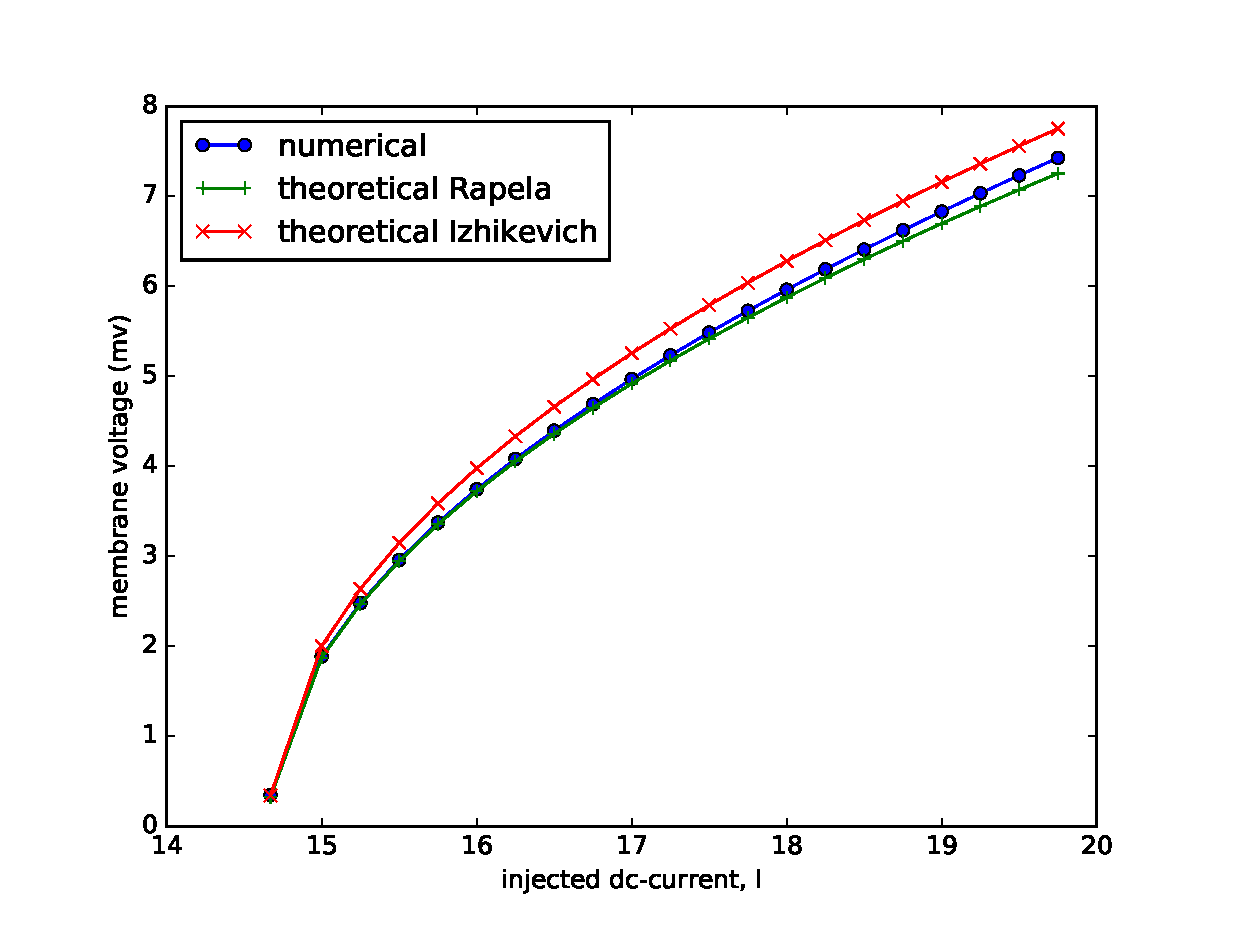
\includegraphics[width=3.75in]{../../figures/ampsFig6-12a-0.0030d-0.0026aI-0.0026dI-0.0029.eps}
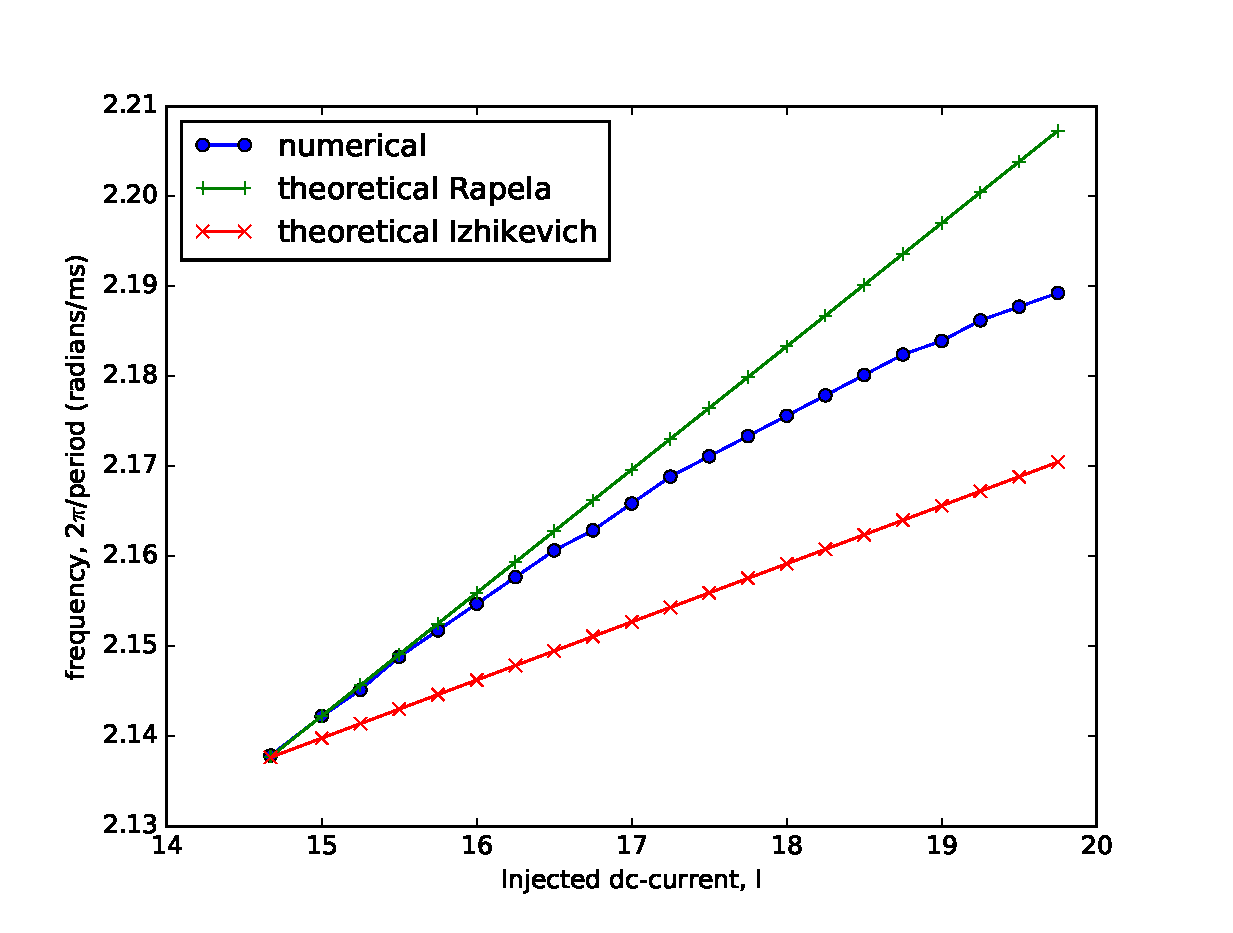
\includegraphics[width=3.75in]{../../figures/freqsFig6-12a-0.0030d-0.0026aI-0.0026dI-0.0029.eps}

\caption{Descriptors (amplitude in panel (a) and frequency in panel (b)) of
limit cycles next to an Andronov-Hopf bifurcation for the $I_{Na,p}+I_K$ model
on the example of page 172 of \citet{izhikevich07} as a function of the input
current to the model. Blue traces give these descriptors values derived from
numerical simulations. Green traces provide theoretical values of these
descriptors, from the formulas given on page 173 of \citet{izhikevich07},
using parameters $a=-0.00297$ and $d=-0.002613$ derived in the previous
section. Red traces are as the green traces but for the parameters $a=0.0026$
and $d=0.0029$ used in the example of page 172 of \citet{izhikevich07}.
Theoretical values obtained using the parameters $a$ and $d$
from the previous section better approximate descriptors derived from
numerical simulations than theoretical values obtained using the parameters in
\citet{izhikevich07}.}

\label{fig:ampsAndFreqsVsIs} 
\end{figure} 
\end{center}

We simulated the $I_{Na,p}+I_K$ model in the example of page 172 of
\citet{izhikevich07} and the topological normal form in Equations~6.8 and 6.9 with the parameters
derived in the previous section and with the parameters in
\citet{izhikevich07}. For these simulations we used a constant injected
dc-current $I=17$.
%
The blue trace in Figure~\ref{fig:voltages} plots voltages from
the $I_{Na,p}+I_K$ model. The green and red traces plot voltages from the 
topological normal forms with the parameters derived in the previous section
and with the parameters in \citet{izhikevich07}, respectively. We see that the
voltages from the topological normal form with the parameters derived in the
previous section better approximate the voltages from the model than the
voltages from the topological normal form with the parameters in
\citet{izhikevich07}.
%
Thus, Figure~\ref{fig:voltages} again shows that the parameters $a$ and $d$ of
the topological normal form in Equations~6.8 and 6.9 derived in the previous
section are more adequate than the ones derived in \citet{izhikevich07}.

\begin{center}
\begin{figure}
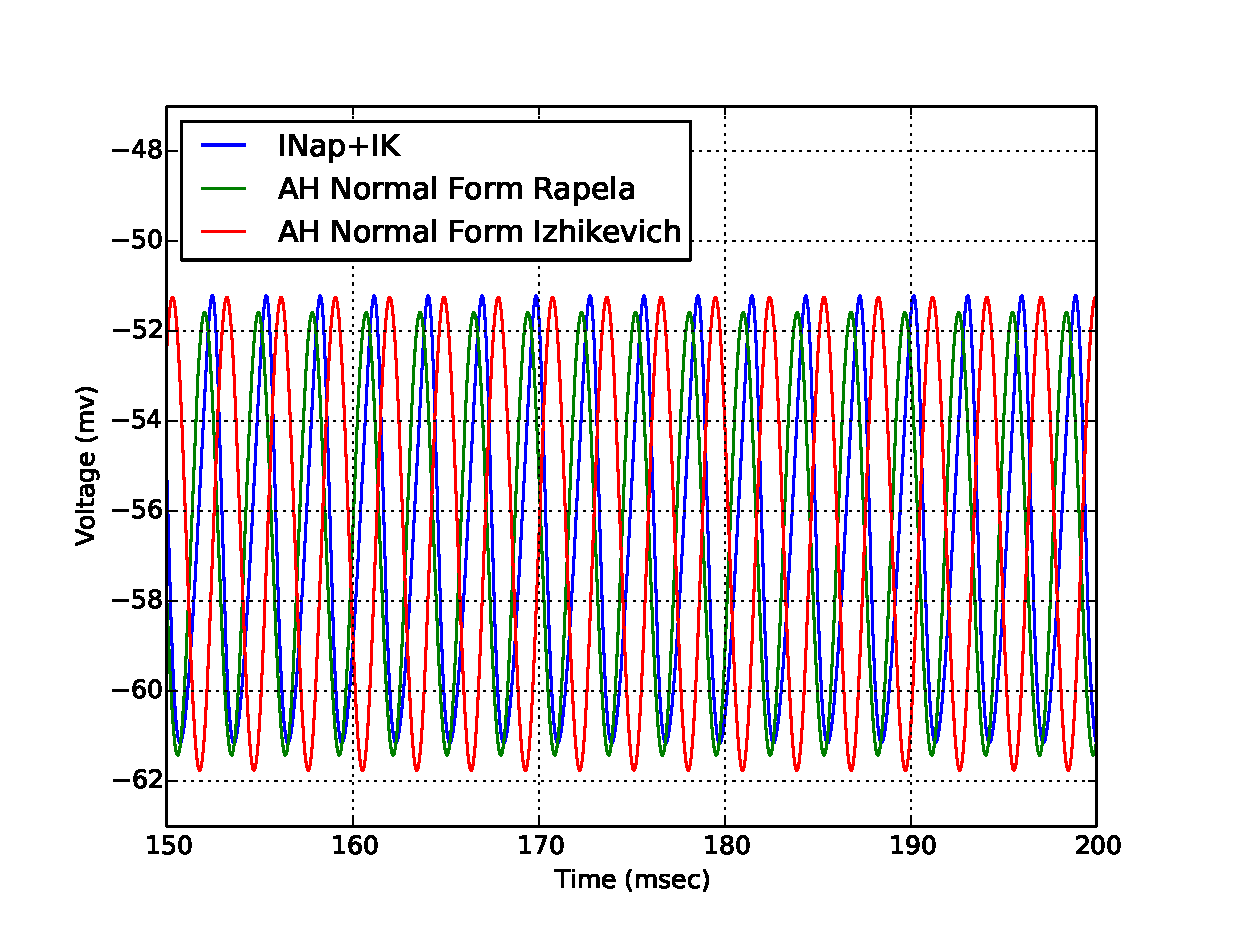
\includegraphics[width=5in]{../../figures/figVoltageExampleP172I17.00a-0.002970d-0.002613aI-0.002600dI-0.002900.eps}

\caption{Voltages from the simulation close to an Andronov-Hopf bifurcation
(input current I=17) of the $I_{Na,p}+I_K$ model on the example of page 172 of
\citet{izhikevich07} and from its topological normal form given in Equations~6.8 and 6.9 of \citet{izhikevich07}. The blue trace gives voltages from
the simulation of the $I_{Na,p}+I_K$ model. The green trace provides voltages
from the simulation of the topological normal form using the parameters
$a=-0.00297$ and $d=-0.002613$ derived in the previous section. The red trace
is as the green one, but for the parameters $a=0.0026$ and $d=0.0029$ used in
the example on page 172 of \citet{izhikevich07}. Voltages from the topological
normal form with the parameters from the previous section are better
approximations to the voltages from the simulation of the $I_{Na,p}+I_K$ model
than voltages from the topological normal form with the parameters used in the
example on page 172 of \citet{izhikevich07}.}

\label{fig:voltages} 
\end{figure} 
\end{center}

\bibliographystyle{apacite}
\bibliography{dynamicalSystems}

\end{document}
